\documentclass[fleqn]{article}
\oddsidemargin 0.0in
\textwidth 6.0in
\thispagestyle{empty}
\usepackage{import}
\usepackage{amsmath}
\usepackage{graphicx}
\usepackage{flexisym}
\usepackage{calligra}
\usepackage{amssymb}
\usepackage{bigints} 
\usepackage[english]{babel}
\usepackage[utf8x]{inputenc}
\usepackage{float}
\usepackage[colorinlistoftodos]{todonotes}


\DeclareMathAlphabet{\mathcalligra}{T1}{calligra}{m}{n}
\DeclareFontShape{T1}{calligra}{m}{n}{<->s*[2.2]callig15}{}
\newcommand{\scriptr}{\mathcalligra{r}\,}
\newcommand{\boldscriptr}{\pmb{\mathcalligra{r}}\,}

\definecolor{hwColor}{HTML}{442020}

\begin{document}

  \begin{titlepage}

    \newcommand{\HRule}{\rule{\linewidth}{0.5mm}}

    \center

    \begin{center}
      
\includegraphics[height=11cm, width=11cm]{asu.png}
    \end{center}

    \vline

    \textsc{\LARGE Statistical/Thermal Physics}\\[1.5cm]

    \HRule \\[0.5cm]
    { \huge \bfseries Homework 8}\\[0.4cm] 
    \HRule \\[1.0cm]

    \textbf{Behnam Amiri}

    \bigbreak

    \textbf{Prof: Michael Treacy}

    \bigbreak

    \textbf{{\large \today}\\[2cm]}

    \vfill

  \end{titlepage}

  \begin{enumerate}
    \item \textbf{5.1} Let the system be one mole of argon gas at romom temperature and atmospheric presure. Compute
    the total energy (kinetic only, neglecting atomic rest energies), entropy, enthalpy, Helmholtz free energy, and 
    Gibbs free energy. Express all answers in SI units.

    \begin{center}
      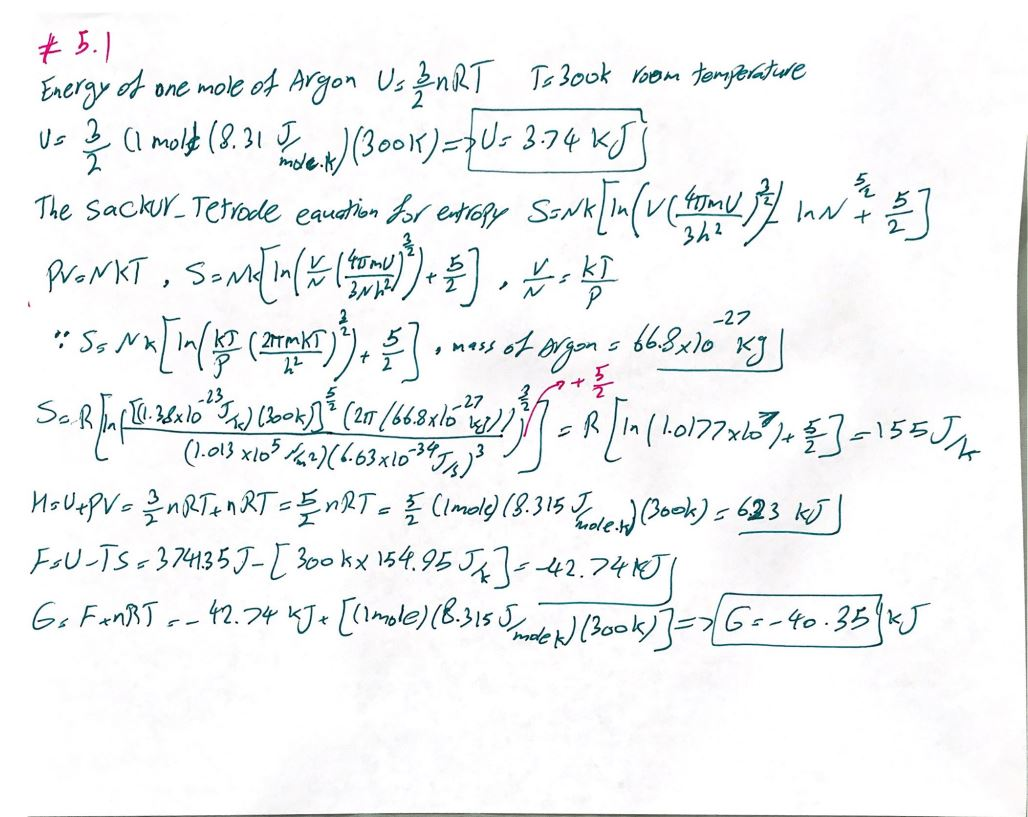
\includegraphics[height=16cm, width=17cm]{51.JPG}
    \end{center}

    \pagebreak

    \item \textbf{5.2} Consider the production of ammonia from nitrogen and hydrogen
    $$
      N_2+3H_2 \longrightarrow 2NH_3,
    $$
    at $298 ~ K$ and $1$ bar. From the values of $\Delta H$ and $S$ tabulated at the back of this book, compute $\Delta G$
    for this reaction and check that it is consistent with the value given in the table.

    \begin{center}
      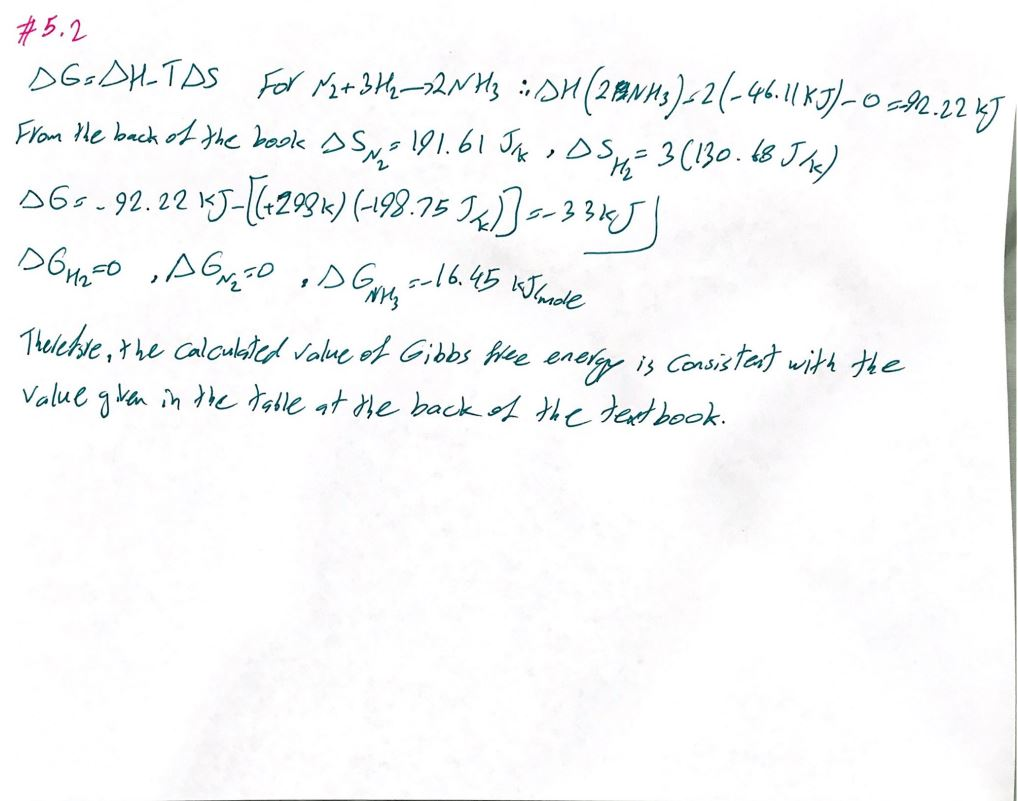
\includegraphics[height=16cm, width=17cm]{52.JPG}
    \end{center}

    \pagebreak

    \item \textbf{5.4} In a hydrogen fuel cell, the steps of the chemical reaction are
    $$
      \text{at - electrode: } H_2+2OH^- \longrightarrow 2H_2O+2e^-
    $$
    $$
      \text{at + electrode: } \dfrac{1}{2} O_2+H_2 O+2e^- \longrightarrow 2OH^-
    $$
    Calculate the voltage of the cell. What is the minimum voltage required for electrolysis of water? Explain briefly.
    
    \begin{center}
      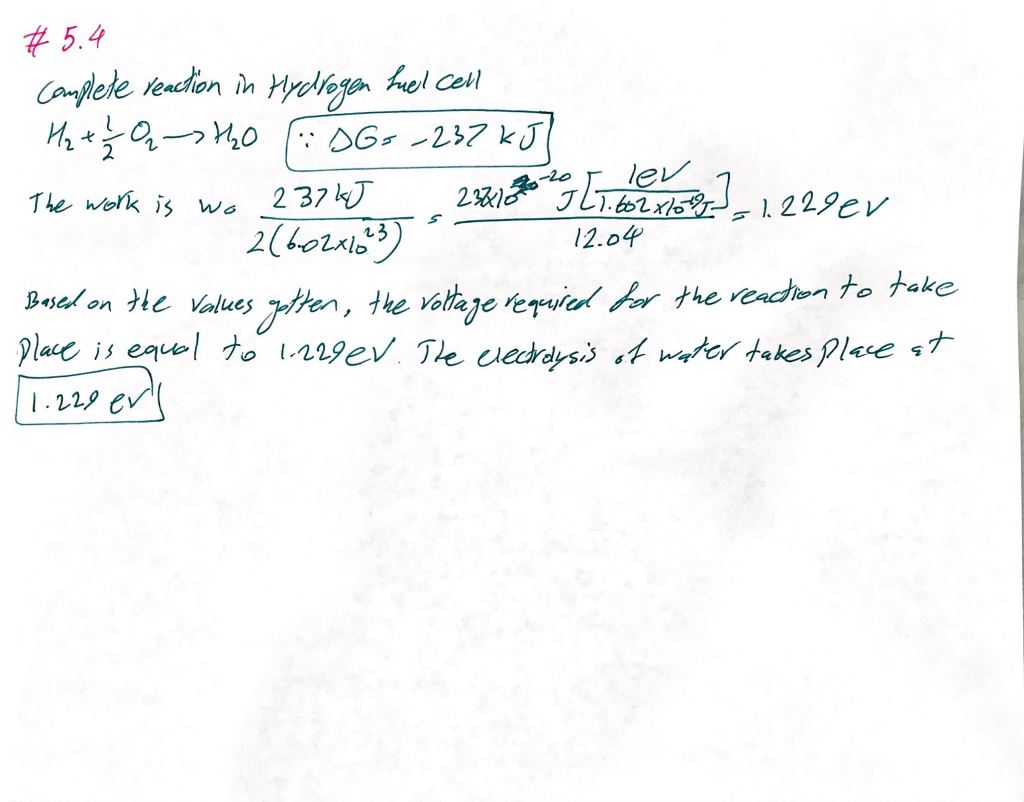
\includegraphics[height=14cm, width=16cm]{54.JPG}
    \end{center}

    \pagebreak

    \item \textbf{5.6} A muscle can be thought of as a fuel cell, producing work from the metabolism of glucose:
    $$
      C_6 H_{12} O_6 \longrightarrow 6 CO_2+6H_2 O
    $$
    \begin{enumerate}
      \item Use the data at the back of this book...

      \item What is the maximum amount of work...

      \item Still assuming ideal operation, how much heat...

      \item Use the concept of entropy to explain why the heat flows in the direction it does.

      \item How would your answers to parts (b) and (c) change, if the operation of muscle is not ideal?

    \end{enumerate}

    \begin{center}
      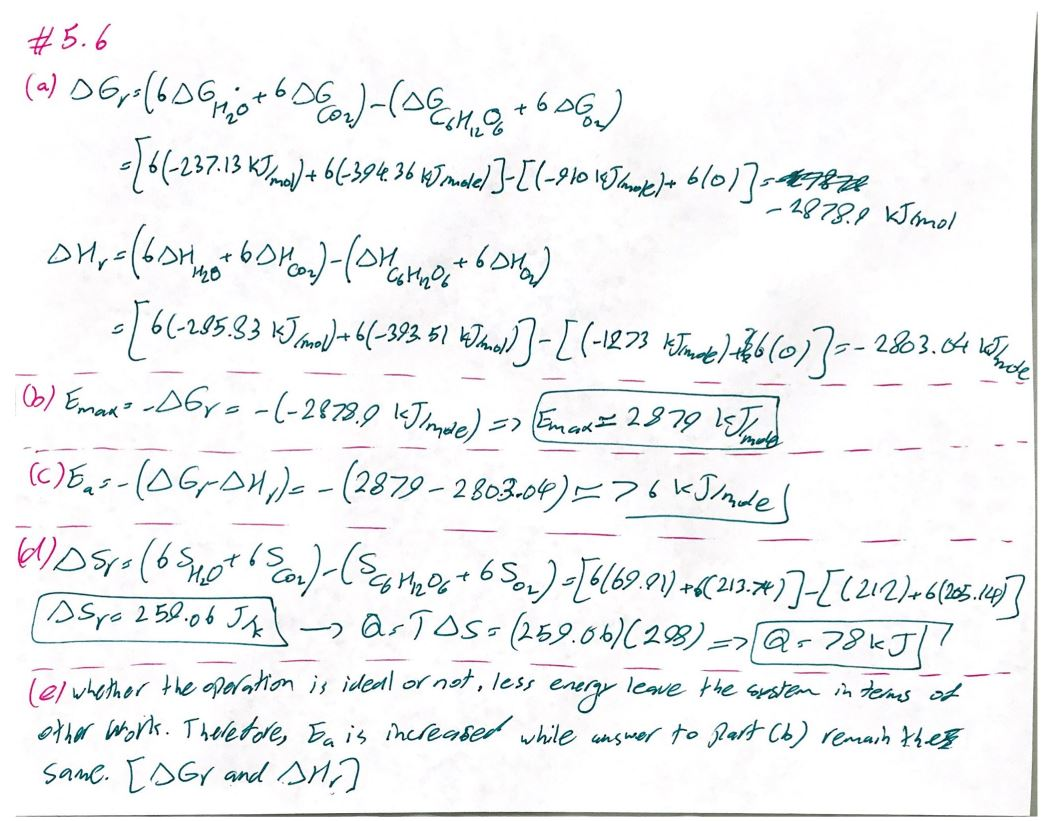
\includegraphics[height=14cm, width=15cm]{56.JPG}
    \end{center}

    \pagebreak

    \item \textbf{5.12} Functions encountered in physics are genrally well enough behaved that their mixed partial 
    derivatives do not depend on which derivative is taken first. Therefore, for instance,
    $$
      \dfrac{\partial}{\partial V} \bigg( \dfrac{\partial U}{\partial S} \bigg)=\dfrac{\partial}{\partial S} \bigg( \dfrac{\partial U}{\partial V} \bigg),
    $$
    where each $\partial/\partial V$ is taken with $S$ fixed, each $\partial/\partial S$ is taken with $V$ fixed, and 
    $N$ is always held fixed...

    \begin{center}
      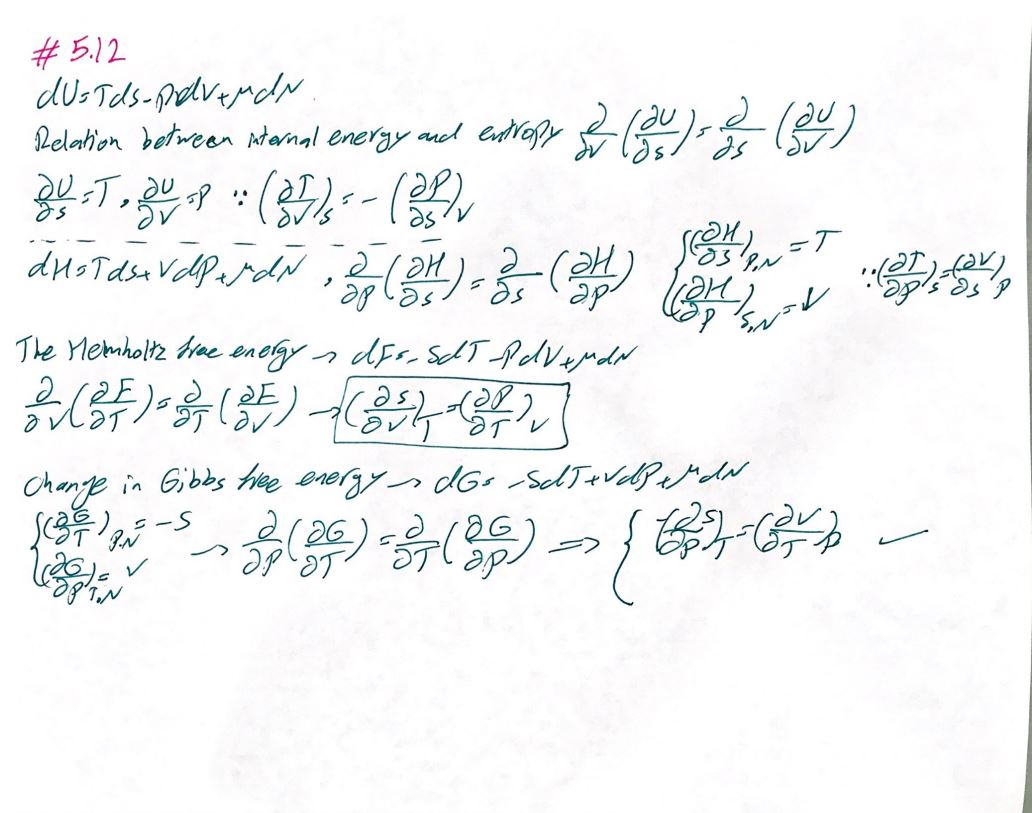
\includegraphics[height=15cm, width=17cm]{512.JPG}
    \end{center}

    \pagebreak

    \item \textbf{5.14} The partial-derivative relatins derived in Problems $1.46, 3.33$ and $5.12$, plus a bit more...
    \begin{enumerate}
      \item With the heat capacity expressions from Problem $3.33$ in mind...

      \item To bring in $C_P$, consider $V$ to be...

      \item Write the remaining partial derivatives in terms...

      \item Check that this formula gives the correct...

      \item Use this formula to argue that $C_P$ cannot be less thatn $C_V$.

      \item Use the data in Problem $1.46$ to evaluate...

      \item Figure $1.14$ shows measured values of $C_P$ for three elemental...

    \end{enumerate}

    \begin{center}
      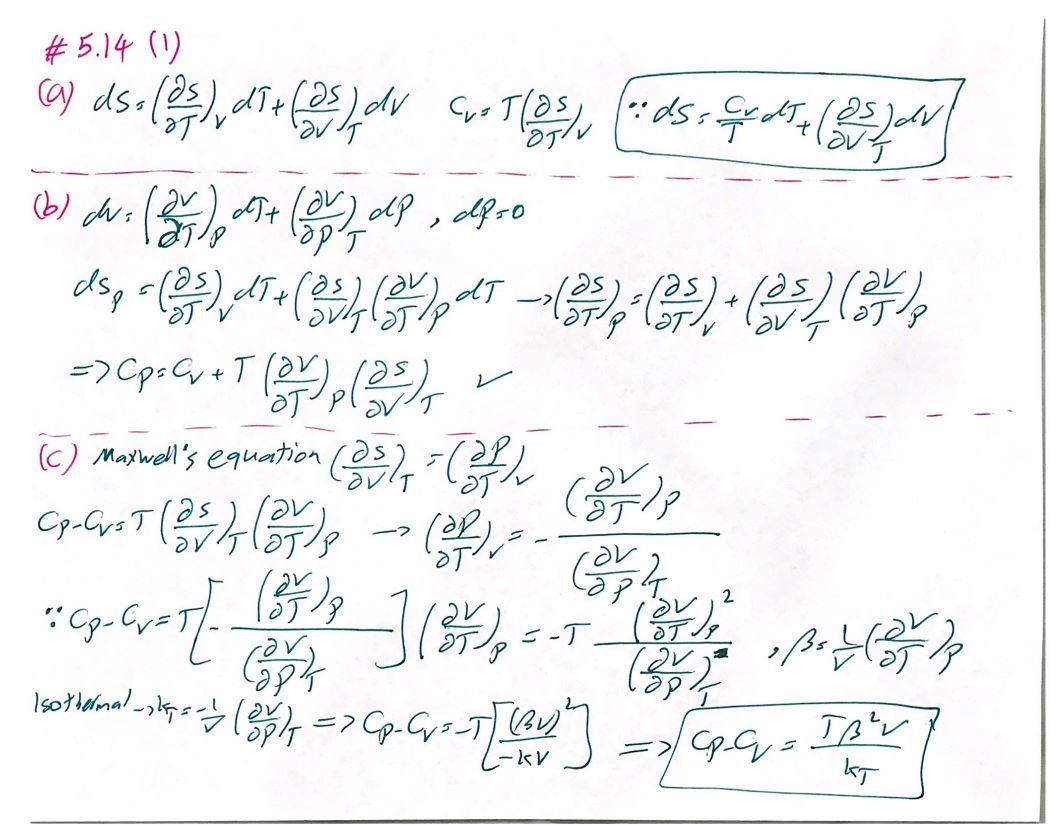
\includegraphics[height=14cm, width=17cm]{514A.JPG}
    \end{center}

    \pagebreak

    \begin{center}
      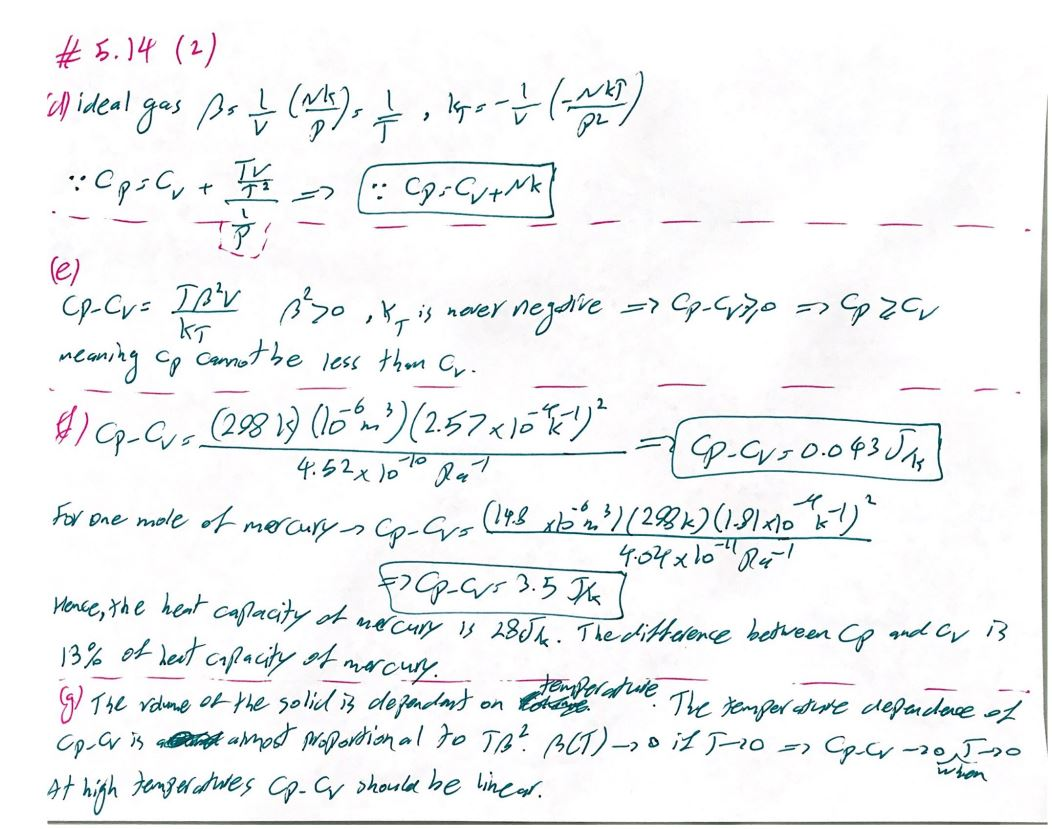
\includegraphics[height=14cm, width=17cm]{514B.JPG}
    \end{center}

  \end{enumerate}

\end{document}
